

\begin{figure*}[ht!]
	\centering
	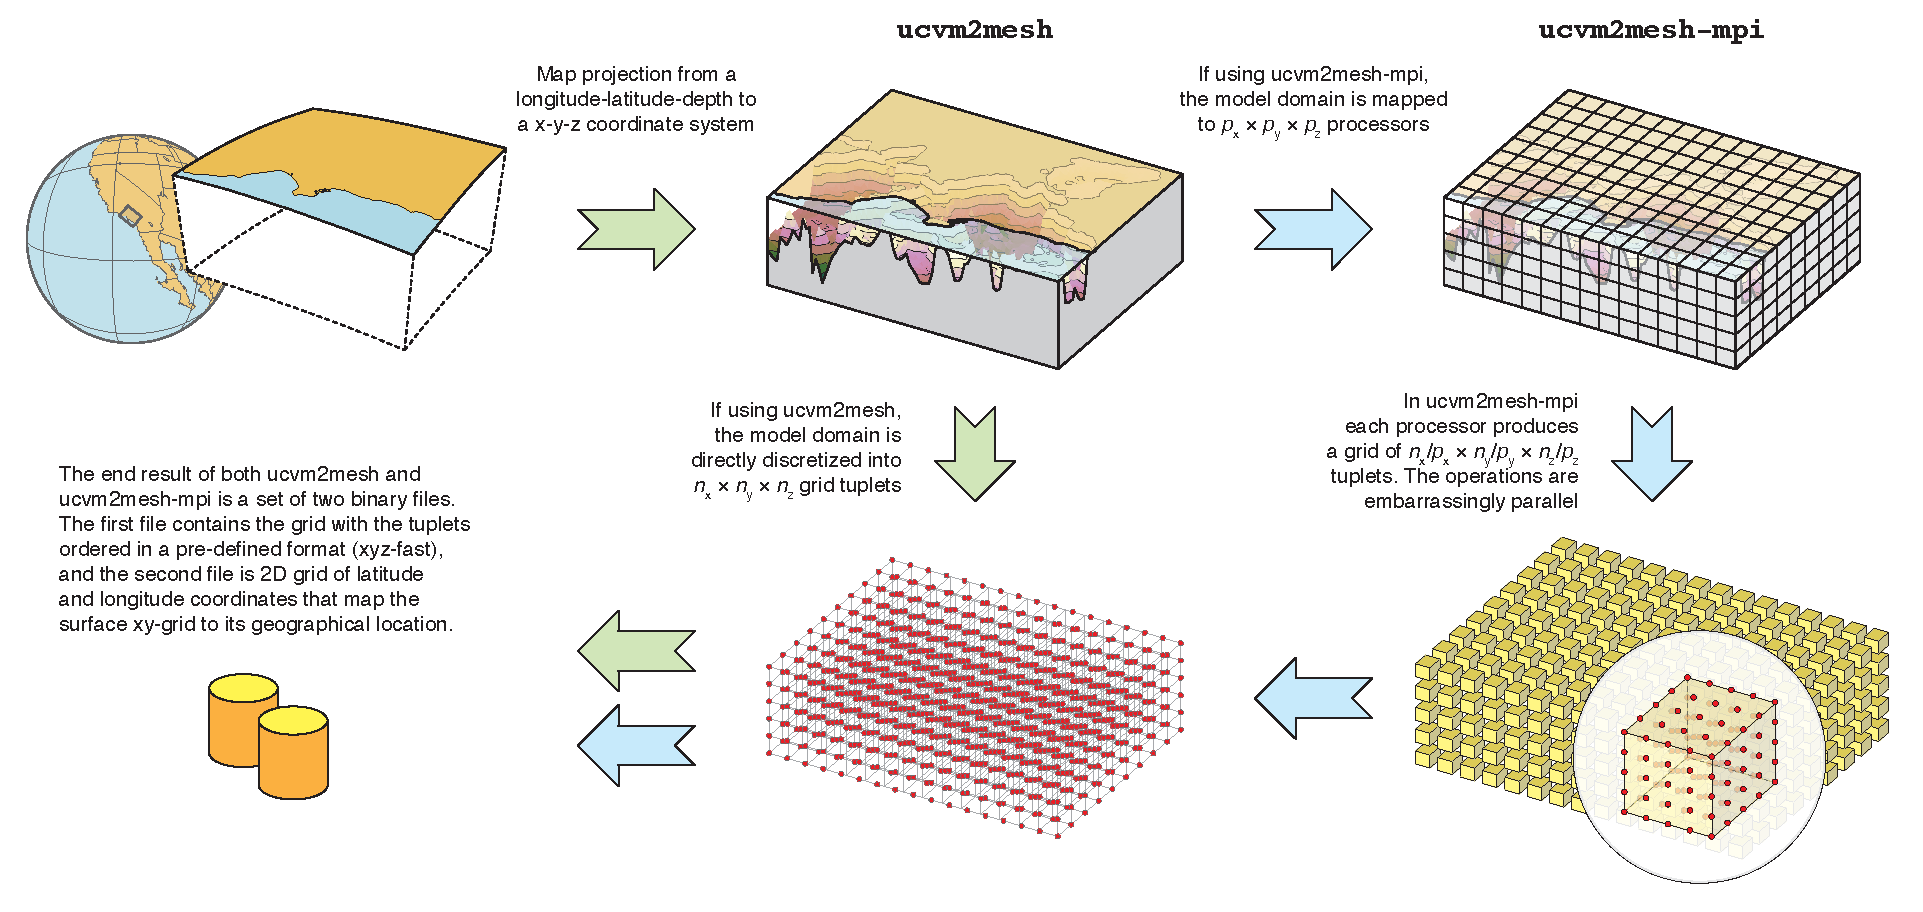
\includegraphics
		[width=\textwidth]
		{figures/pdf/ucvm-to-mesh}
	\caption{Construction of a structured grid with the programs \texttt{ucvm2mesh} (green arrows) and \texttt{ucvm2mesh-mpi} (blue arrows). An important aspect of the gridding process is that the discretized information payload (\vs{}, \vp{}, and $\rho$) is stored at the grid points. That is, the querying and assignment process has a 1-to-1 mapping between the queried point and the grid node of the mesh.}
	\label{fig:meshing}
\end{figure*}


\subsection{Creating Structured 3D Meshes}

One of the most important features of UCVM is that the framework can be used to generate uniform grids (here also referred as structured meshes) in a format consistent with that used by the AWP-ODC simulation code \citep{Cui_2010_Proc}. This feature is supported through the program \texttt{ucvm2mesh}.

Construction of a mesh proceeds as shown in Figure \ref{fig:meshing}. The user specifies a two-dimensional map projection (such as UTM-11), a latitude and longitude geographic anchor point, mesh cell dimensions ($n_x$, $n_y$, $n_z$) along the $x$, $y$ and $z$ axes (where the $x,y$ coordinates define the plane of the projection and $z$ is the vertical component), step size $d_x$ in meters within the projected space, and rotation angle within the map projection. Additionally, the user provides a list of CVMs to query. These models are then tiled by the program as described above.

The program \texttt{ucvm2mesh} projects the geographic coordinates of the Earth's surface into the map projection, placing the origin of the mesh as the anchor point and discretizing the volume according to the provided dimensions and step size. For each point in the projected volume, \texttt{ucvm2mesh} determines the analogous geographic point in terms of latitude, longitude and depth, and queries the underlying CVMs for material properties. These material properties are then assigned to the mesh point. In the process, a minimum \vs{} floor can also be set to bound lower velocities.

The program outputs two binary files. The first file represents the extracted mesh and consists of a list of $n_xn_yn_z$ tuples. Each tuple contains three single precision floating point values (\vp{}, \vs{}, $\rho$), representing the material properties for a point in the mesh, with the mesh coordinates given implicitly by the position of the tuple in the list. The tuples are arranged in $x$-$y$-$z$ order, with units of m/s for the velocities and kg/m$^3$ for the density. The second file contains a $(n_x \times n_y)$ grid of latitude and longitude coordinates corresponding to the geographic location of the surface grid points within the mesh. This metadata is useful for visualization purposes.

To facilitate the construction of very large meshes, the framework also offers a parallel version of the mesher named \texttt{ucvm2mesh-mpi}. This MPI program operates analogously to that of the serial version (see Figure \ref{fig:meshing}). Spatial decomposition is performed by mapping subblocks of the meshing region to individual processors for extraction. The mapping is specified by providing a processor grid to the program at startup, which specifies the number of processors along each dimension. If the meshing region is sized $(n_x \times n_y \times n_z)$ grid points along each dimension, and the processor grid is specified as ($p_x$, $p_y$, $p_z$), then each processor is assigned $(n_x/p_x \times n_y/p_y \times n_z/p_z)$ grid points. The only constraint in the mapping is that the processor count along a particular dimension must divide evenly into the number of grid points along that dimension. Once the region has been decomposed in this manner, extraction of material properties is an embarrassingly parallel operation.  
